% PREAMBLE
\documentclass[11pt]{amsart}
\usepackage[T1]{fontenc}
\usepackage{lmodern}
\usepackage{microtype}
\usepackage{amsmath,amssymb}
\usepackage{mathtools}
\usepackage{graphicx}
\usepackage{booktabs}
\usepackage{tikz}
\usepackage[colorlinks=true,linkcolor=blue!45!black,citecolor=blue!45!black,urlcolor=blue!45!black]{hyperref}
\usepackage[capitalize]{cleveref}

\emergencystretch=3em

\newtheorem{theorem}{Theorem}[section]
\newtheorem{proposition}[theorem]{Proposition}
\newtheorem{lemma}[theorem]{Lemma}
\newtheorem{corollary}[theorem]{Corollary}
\newtheorem{conjecture}[theorem]{Conjecture}
\theoremstyle{definition}
\newtheorem{definition}[theorem]{Definition}
\newtheorem{fact}[theorem]{Fact}
\newtheorem{quoted}[theorem]{Quoted}
\theoremstyle{remark}
\newtheorem{remark}[theorem]{Remark}

\title[A Power Saving for M\"obius Sums on Missing-Digit Integers]{A Power Saving for M\"obius Sums on Missing-Digit Integers, under GRH}
\author{Carlo Mitchener}
\address{MrlyProd, Inc.}
\email{carlo.mitchener@gmail.com}
\date{First published 2026-09-06}

% PAPER
\begin{document}

\begin{abstract}
Take the whole numbers whose base expansion never uses one chosen digit, and add up the M\"obius function over the ones below a given bound. The trivial estimate for that sum is the number of terms, and among the sources we read we find nothing better. Assuming the generalized Riemann hypothesis we beat it by a fixed power, for every base $q \ge 3690$ with one digit removed: writing $A_F(x)$ for the count of such integers up to $x$ and $M_F(x)$ for the M\"obius sum over them, $M_F(x) \ll_{q,\delta'} A_F(x)^{1-\delta'}$ for every fixed $\delta' < \delta_q$, where $\delta_q$ is explicit and tends to $1/4$ as the base grows. The proof expands the digit indicator into additive frequencies, pays one $\ell^1$ norm for the expansion, and quotes one published exponential-sum bound at each frequency; the content is that past a computable base the norm costs less than the set's own mass. The same five steps run on any zero-free half plane for Dirichlet $L$-functions, at a base we compute for each. We also prove the wall: that $\ell^1$ norm can never be smaller than one, so the argument yields nothing unconditional and nothing at all about digit sets of fewer than $q^{3/4}$ digits.
\end{abstract}

% TITLE PAGE
\makeatletter
\global\let\titledate\@date
\global\let\paperabstract\@setabstracta
\global\let\@date\@empty
\global\let\@setabstract\relax
\makeatother

\maketitle

\begin{center}
\normalfont\footnotesize\titledate
\end{center}

\vspace*{\stretch{1}}

\begin{center}

\includegraphics[width=0.5\textwidth]{figures/avatar.png}
\end{center}

\vspace*{\stretch{1.25}}

\newpage

\paperabstract

% BODY
\section{Introduction}
\label{sec:intro}

Fix a base $q$ and throw away one digit. In base ten with the digit $7$ removed, what is left is
\[
  1,\,2,\,3,\,4,\,5,\,6,\,8,\,9,\,10,\,\dots,\,16,\,18,\,\dots,\,69,\,80,\,81,\,\dots
\]
and the pattern continues forever, thinning as the numbers get longer: below $10^n$ there are about $9^n$ of them instead of $10^n$. Sets like this are called \emph{missing-digit} or \emph{ellipsephic} sets. They are sparse, they are easy to describe, and they are famously hard to do arithmetic on, because knowing the digits of $n$ tells you almost nothing about the primes dividing $n$.

Now put the M\"obius function on them. Recall that $\mu(n)$ is $0$ when $n$ has a repeated prime factor, and otherwise $+1$ or $-1$ according to whether $n$ has an even or an odd number of prime factors. Summing $\mu$ over all integers up to $x$ gives Mertens' function, and how much it cancels is the Riemann hypothesis. Summing it over the missing-digit integers up to $x$ gives
\[
  M_F(x) = \sum_{\substack{n \le x \\ n \text{ misses the digit}}} \mu(n),
\]
and the question is the same one: does it cancel? The number of terms is $A_F(x)$, of size $x^{\log_q(q-1)}$, and $|M_F(x)| \le A_F(x)$ is free. We looked for anything better in the literature and found no bound on this sum at all; the subsection \emph{Where this sits} below says exactly what we searched, and what we found there instead.

This paper proves a power saving over the free bound, on the generalized Riemann hypothesis, for every base from $3690$ up.

\begin{figure}[h]
\centering
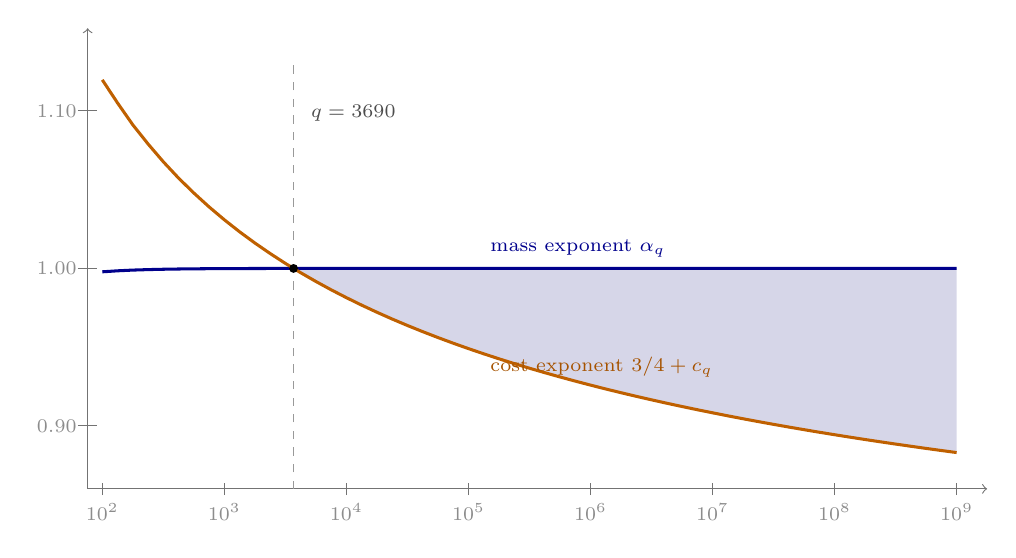
\begin{tikzpicture}[x=1.55cm,y=1cm]
  \fill[blue!45!black,opacity=0.16] (1.5670,2.7993) -- (1.6250,2.7453) -- (1.7500,2.6338) -- (1.8750,2.5282) -- (2.0000,2.4282) -- (2.1250,2.3332) -- (2.2500,2.2429) -- (2.3750,2.1569) -- (2.5000,2.0749) -- (2.6250,1.9966) -- (2.7500,1.9217) -- (2.8750,1.8499) -- (3.0000,1.7812) -- (3.1250,1.7152) -- (3.2500,1.6518) -- (3.3750,1.5908) -- (3.5000,1.5321) -- (3.6250,1.4756) -- (3.7500,1.4211) -- (3.8750,1.3685) -- (4.0000,1.3177) -- (4.1250,1.2686) -- (4.2500,1.2211) -- (4.3750,1.1752) -- (4.5000,1.1307) -- (4.6250,1.0875) -- (4.7500,1.0457) -- (4.8750,1.0052) -- (5.0000,0.9658) -- (5.1250,0.9275) -- (5.2500,0.8904) -- (5.3750,0.8542) -- (5.5000,0.8191) -- (5.6250,0.7849) -- (5.7500,0.7516) -- (5.8750,0.7192) -- (6.0000,0.6876) -- (6.1250,0.6568) -- (6.2500,0.6267) -- (6.3750,0.5974) -- (6.5000,0.5688) -- (6.6250,0.5409) -- (6.7500,0.5136) -- (6.8750,0.4870) -- (7.0000,0.4610) -- (7.0000,2.8000) -- cycle;
  \draw[->,black!55] (-0.12,0) -- (7.25,0);
  \draw[->,black!55] (-0.12,0) -- (-0.12,5.85);
  \foreach \x/\l in {0/2, 1/3, 2/4, 3/5, 4/6, 5/7, 6/8, 7/9} {
    \draw[black!55] (\x,-0.08) -- (\x,0.08) node[below=4pt,font=\scriptsize,black!45] {$10^{\l}$};
  }
  \foreach \y/\l in {0.8/0.90, 2.8/1.00, 4.8/1.10} {
    \draw[black!55] (-0.2,\y) -- (-0.04,\y) node[left=4pt,font=\scriptsize,black!45] {$\l$};
  }
  \draw[dashed,black!40] (1.5670,0) -- (1.5670,5.4);
  \draw[line width=1.1pt,blue!55!black] (0.0000,2.7564) -- (0.1250,2.7691) -- (0.2500,2.7783) -- (0.3750,2.7845) -- (0.5000,2.7890) -- (0.6250,2.7922) -- (0.7500,2.7944) -- (0.8750,2.7960) -- (1.0000,2.7971) -- (1.1250,2.7979) -- (1.2500,2.7985) -- (1.3750,2.7989) -- (1.5000,2.7992) -- (1.6250,2.7994) -- (1.7500,2.7996) -- (1.8750,2.7997) -- (2.0000,2.7998) -- (2.2500,2.7999) -- (2.5000,2.7999) -- (2.7500,2.8000) -- (3.0000,2.8000) -- (4.0000,2.8000) -- (5.0000,2.8000) -- (6.0000,2.8000) -- (7.0000,2.8000);
  \draw[line width=1.1pt,orange!75!black] (0.0000,5.1943) -- (0.1250,4.9008) -- (0.2500,4.6232) -- (0.3750,4.3802) -- (0.5000,4.1539) -- (0.6250,3.9466) -- (0.7500,3.7573) -- (0.8750,3.5808) -- (1.0000,3.4173) -- (1.1250,3.2647) -- (1.2500,3.1225) -- (1.3750,2.9891) -- (1.5000,2.8635) -- (1.6250,2.7453) -- (1.7500,2.6338) -- (1.8750,2.5282) -- (2.0000,2.4282) -- (2.1250,2.3332) -- (2.2500,2.2429) -- (2.3750,2.1569) -- (2.5000,2.0749) -- (2.6250,1.9966) -- (2.7500,1.9217) -- (2.8750,1.8499) -- (3.0000,1.7812) -- (3.1250,1.7152) -- (3.2500,1.6518) -- (3.3750,1.5908) -- (3.5000,1.5321) -- (3.6250,1.4756) -- (3.7500,1.4211) -- (3.8750,1.3685) -- (4.0000,1.3177) -- (4.1250,1.2686) -- (4.2500,1.2211) -- (4.3750,1.1752) -- (4.5000,1.1307) -- (4.6250,1.0875) -- (4.7500,1.0457) -- (4.8750,1.0052) -- (5.0000,0.9658) -- (5.1250,0.9275) -- (5.2500,0.8904) -- (5.3750,0.8542) -- (5.5000,0.8191) -- (5.6250,0.7849) -- (5.7500,0.7516) -- (5.8750,0.7192) -- (6.0000,0.6876) -- (6.1250,0.6568) -- (6.2500,0.6267) -- (6.3750,0.5974) -- (6.5000,0.5688) -- (6.6250,0.5409) -- (6.7500,0.5136) -- (6.8750,0.4870) -- (7.0000,0.4610);
  \fill[black] (1.5670,2.7993) circle (1.6pt);
  \node[font=\scriptsize,anchor=west,blue!55!black] at (3.1,3.05) {mass exponent $\alpha_q$};
  \node[font=\scriptsize,anchor=west,orange!65!black] at (3.1,1.55) {cost exponent $3/4 + c_q$};
  \node[font=\scriptsize,anchor=south west,black!70] at (1.63,4.55) {$q = 3690$};
\end{tikzpicture}
\caption{The whole theorem is this crossing. The horizontal axis is the base. The upper curve is the mass exponent $\alpha_q = \log_q(q-1)$, the size of the missing-digit set as a power of $x$; it climbs towards $1$ and is flat at this scale. The falling curve is what the method costs, $3/4$ from the quoted M\"obius bound plus $c_q$ for the Fourier expansion. Where cost drops below mass, the bound beats the number of terms, and the shaded wedge is the saving. The crossing happens once, at $q = 3690$, and never comes back.}
\label{fig:crossing}
\end{figure}

\subsection*{What is proved}

Write $F$ for the surviving digits, $S_F$ for the integers all of whose base-$q$ digits lie in $F$, $A_F(x) = \#\{n \in S_F : n \le x\}$ and $M_F(x) = \sum_{n \in S_F,\, n \le x} \mu(n)$. Write $\alpha_q = \log_q(q-1)$, so that $A_F(x)$ has order $x^{\alpha_q}$. \Cref{thm:main} says: assume the generalized Riemann hypothesis for Dirichlet $L$-functions; then for every $q \ge 3690$, every $F$ missing exactly one digit and every $\varepsilon > 0$,
\[
  |M_F(x)| \ll_{q,\varepsilon} x^{3/4 + c_q + \varepsilon} \qquad (x \ge 2),
\]
with $3/4 + c_q < \alpha_q$, so that the bound is a power saving against the set's own size: $|M_F(x)| \ll_{q,\delta'} A_F(x)^{1 - \delta'}$ for every fixed $\delta' < \delta_q = (\alpha_q - 3/4 - c_q)/\alpha_q$. The constant $c_q$ is completely explicit, it is the only thing in the statement that is not standard, and it tends to $0$: as the base grows, $\delta_q \to 1/4$ and the bound approaches $A_F(x)^{3/4 + o(1)}$, which is the exponent the generalized Riemann hypothesis gives on the whole line, transplanted onto the sparse set and measured against the sparse set's own mass.

Two warnings belong in the same breath as the theorem, and they are repeated wherever it is restated. The implied constant depends on $q$; nothing here is uniform in the base. And $\delta_q$ is fixed before $\varepsilon$ is chosen, so what is proved is $A_F(x)^{1-\delta'}$ for each fixed $\delta' < \delta_q$ and never the endpoint $A_F(x)^{1 - \delta_q}$. At $q = 3690$ that distinction is the whole claim, because there $\delta_q$ is only $5.863 \times 10^{-6}$.

\subsection*{The proof in one paragraph}

The indicator of a length-$L$ digit string over $F$ expands into additive characters modulo $q^L$, and because digits are independent the Fourier coefficient factors over digit positions:
\[
  \widehat F_L(t) = \prod_{j < L} g_F(q^j t), \qquad g_F(t) = \sum_{d \in F} e(dt).
\]
Expanding $M_F(x)$ this way turns it into
\[
  q^{-L} \sum_{a \bmod q^L} \widehat F_L(a/q^L) \sum_{n \le x} \mu(n) e(-na/q^L),
\]
so the whole sum is bounded by the $\ell^1$ norm of the transform times the largest M\"obius exponential sum. Under the generalized Riemann hypothesis that largest sum is $x^{3/4+\varepsilon}$, uniformly in the frequency, by a theorem of Baker and Harman \cite{bh}. The $\ell^1$ norm obeys a one-step recursion: peeling off the last digit costs a single constant $B_q(F) = \sup_t \sum_{r \bmod q} |g_F((t+r)/q)|$ per digit, so the normalised norm is at most $(B_q(F)/q)^L = q^{L c_q}$. What remains is to bound $B_q(F)$ explicitly, and that is elementary trigonometry on a grid of $q$ equally spaced points: the Dirichlet kernel contributes at most $\Phi_q \approx (2/\pi) q \ln q$, and the one missing digit contributes at most $q$ by an exact Parseval identity. Then $c_q = \log_q(1 + \Phi_q/q)$ is of size $\ln\ln q/\ln q$, and the arithmetic of \cref{fig:crossing} does the rest.

Nothing in that chain except the quoted M\"obius bound depends on the exponent $3/4$. So the same five steps run on any hypothesis of the form ``no Dirichlet $L$-function vanishes in $\sigma > a$'', with the exponent $b(a)$ that Baker and Harman \cite{bh} and Zhang \cite{zhang} attach to it, and the price of a weaker hypothesis is paid entirely in the base: \cref{thm:ladder} and the rungs of \cref{fact:ladder}. A zero-free half plane at $\sigma > 19/20$ still buys the saving, at a base with $84$ decimal digits.

\subsection*{Where this sits}

Missing-digit sets carry a serious literature, and the arithmetic functions it has reached do not include $\mu$. Erd\H{o}s, Mauduit and S\'ark\"ozy \cite{ems} and Konyagin \cite{konyagin} study their distribution in residue classes; Dartyge and Mauduit \cite{dm} get almost primes; Maynard \cite{maynard19} proves there are infinitely many primes missing a digit in base ten, and \cite{maynard22} extends that to large bases with many digits missing; Nath \cite{nath} proves Bombieri-Vinogradov theorems for $\Lambda(n) 1_A(n)$; Leng and Sawhney \cite{ls} settle ternary Goldbach on such a set; Kim \cite{kim} computes the divisor function over one. In every one of these the set enters through the Fourier norms of its digit transform, exactly as it does here.

What we could not find anywhere is the M\"obius sum itself. A whole-text search of \cite{maynard19}, \cite{maynard22} and \cite{nath} finds the word ``M\"obius'' once in about three thousand lines, as an inversion step inside a proof, ``Liouville'' nowhere, and ``Mertens'' only as Mertens' theorem on a product over primes. So we state the positioning as a search and not as a non-existence result: those three full texts were read at their sources and searched end to end, the rest of the bibliography was read for its statements, and in none of them do we find a bound on $\sum_{n \le x,\, n \in S_F} \mu(n)$; \cref{thm:main} appears to be the first. The card it claims is precise, and each coordinate on it matters: the sequence is $\mu$ restricted to $S_F$; the norm is a pointwise bound in $x$, with no averaging and no modulus; the range is $q \ge 3690$ with one digit removed; and the saving is a fixed power of the set's own counting function, conditional on the generalized Riemann hypothesis. Change any coordinate and the claim is not ours.

One thing the reader should not conclude is that the \emph{shape} of such a result is new. Maynard \cite{maynard22} records in his own paper that his asymptotic for $\sum_{n < q^k} \Lambda(n) 1_A(n)$ has error terms that ``could be replaced by effective ones of size $O((q-1)^k \exp(-c k^{1/2}))$'', because the moduli occurring are highly composite and Siegel zeros do not intervene. A saving of that shape over a missing-digit set is therefore already in print, for $\Lambda$. What is different here is the function, and what is worse here is the hypothesis.

\subsection*{What this does not do, and cannot}

The method has a floor, and we prove it rather than guess it. For \emph{every} digit set, an exact Parseval identity on the shifted grid gives $\sum_{r \bmod q} |g_F((t+r)/q)|^2 = qk$, whence $B_q(F) \ge q$ and $c_q \ge 0$ (\cref{thm:floor}). The $\ell^1$ recursion therefore never contracts, and three consequences follow at once. The decomposition needs $\alpha_q > 3/4$, that is more than $q^{3/4}$ surviving digits, so it says nothing whatever about a set like $\{0,1\}$ in base $3$. Put Davenport's unconditional bound into the quoted step instead of the conditional one and the answer exceeds $A_F(x)$: no unconditional theorem hides inside this argument. And rearranging the same two factors by Cauchy-Schwarz instead is worse than trivial.

That is the honest picture: a dense-column theorem, conditional, with a proved wall on both sides of it. \Cref{sec:open} lists what it leaves undone.

\section{Definitions}
\label{sec:defs}

Throughout, $e(t) = e^{2\pi i t}$, $\|t\|$ is the distance from $t$ to the nearest integer, $\gamma = 0.5772156649\ldots$ is Euler's constant, and $\mu$ is the M\"obius function. All implied constants are made explicit where they matter and are otherwise absolute unless a subscript says otherwise.

\begin{definition}[The set, its mass, its meter]
\label{def:set}
Fix an integer base $q \ge 3$ and a set $E \subseteq \{0, 1, \dots, q-1\}$ of \emph{excluded digits}, with $m = |E| \ge 1$. Put $F = \{0,1,\dots,q-1\} \setminus E$ and $k = |F| = q - m$. Let
\[
  S_F = \{ n \ge 1 : \text{every base-$q$ digit of $n$ lies in } F \},
\]
and write $A_F(x) = \#\{n \in S_F : n \le x\}$ for its counting function and
\[
  M_F(x) = \sum_{\substack{n \in S_F \\ n \le x}} \mu(n)
\]
for the M\"obius sum over it. The \emph{mass exponent} is $\alpha_q = \log_q k$. Counting digit strings gives $A_F(q^L) \ge k^L - 1$ and hence $A_F(x) \gg_q x^{\alpha_q}$ for all $x \ge q$, so $\alpha_q$ is the exponent of the set.
\end{definition}

\begin{definition}[The digit symbol and the level transform]
\label{def:transform}
The \emph{digit symbol} of $F$ is $g_F(t) = \sum_{d \in F} e(dt)$, and $D_q(t) = \sum_{d=0}^{q-1} e(dt)$ is the full Dirichlet kernel, so that $|D_q(t)| = |\sin(\pi q t)/\sin(\pi t)|$ for $t \notin \mathbb Z$. Let $\mathcal D_L$ be the set of integers $\sum_{j<L} f_j q^j$ with every $f_j \in F$, that is the values of the length-$L$ digit strings over $F$, leading zeros allowed. The \emph{level-$L$ transform} is
\[
  \widehat F_L(t) = \sum_{n \in \mathcal D_L} e(nt) = \prod_{j<L} g_F(q^j t),
\]
the product formula holding because the digits of a string are chosen independently.
\end{definition}

\begin{definition}[The one-step constant and the proved bound]
\label{def:const}
The \emph{one-step constant} of the shifted-grid recursion is
\[
  B_q(F) = \sup_{t \in \mathbb R} \ \sum_{r \bmod q} \Bigl| g_F\Bigl(\frac{t+r}{q}\Bigr) \Bigr| .
\]
Write $H(n) = \ln n + \gamma + \frac{1}{2n}$ for the standard upper bound on the $n$-th harmonic number, and set
\[
  \Phi_q = \frac{4}{\pi} q + \frac{2q}{\pi} H\Bigl( \Bigl\lceil \frac{q-2}{2} \Bigr\rceil \Bigr) + \Bigl( 1 - \frac{2}{\pi} \Bigr)(q-2) + 0.727,
  \qquad
  P_q(m) = \sqrt m + \frac{\Phi_q}{q} .
\]
\Cref{lem:kernel} proves $B_q(F) \le q\,P_q(m)$ for every $F$ with $|E| = m$. The \emph{cost exponent} is
\[
  c_q = \log_q P_q(m),
\]
defined from the proved bound $P_q(m)$ and never from the exact supremum $B_q(F)$; when $m$ is not $1$ we write $c_q(m)$. Note $\Phi_q = \frac{2}{\pi} q \ln q\,(1 + o(1))$, so $c_q = \bigl(\ln\ln q + \ln(2/\pi) + o(1)\bigr)/\ln q$.
\end{definition}

\begin{definition}[The saving and the certificate]
\label{def:saving}
For $m$ excluded digits put
\[
  \delta_q = \frac{\alpha_q - 3/4 - c_q}{\alpha_q},
  \qquad
  \operatorname{gap}_q(m) = k q^{-3/4} - P_q(m) .
\]
Since $\alpha_q - 3/4 - c_q = \log_q\bigl(k q^{-3/4} / P_q(m)\bigr)$, the two tests agree: $3/4 + c_q < \alpha_q$ if and only if $\operatorname{gap}_q(m) > 0$, and
\begin{equation}
  \label{eq:cancelfree}
  \delta_q = \frac{\ln\bigl(1 + \operatorname{gap}_q(m)/P_q(m)\bigr)}{\alpha_q \ln q} .
\end{equation}
Form \eqref{eq:cancelfree} never differences two numbers of size $1$ to produce one of size $10^{-6}$, and it is the form every printed $\delta_q$ margin below is computed from; the $\operatorname{gap}_q$ margins are the difference itself, which is what they are.
\end{definition}

\begin{definition}[The zero-free hypothesis and the exponent it buys]
\label{def:zfree}
For $\tfrac12 \le a < 1$, let $Z(a)$ be the hypothesis that $L(s,\chi)$ has no zero in the half plane $\sigma > a$, for every Dirichlet character $\chi$ of every modulus. Thus $Z(1/2)$ is the generalized Riemann hypothesis in its Dirichlet form. Let
\[
  b(a) = \min\bigl( b_{\mathrm{BH}}(a),\, b_{\mathrm Z}(a) \bigr),
  \qquad
  b_{\mathrm{BH}}(a) =
  \begin{cases}
    a + 1/4, & 1/2 \le a < 11/20, \\
    4/5, & 11/20 \le a < 3/5, \\
    (a+1)/2, & 3/5 \le a < 1,
  \end{cases}
\]
with $b_{\mathrm Z}(a) = (8a - 7a^2)/(4 - 2a)$ for $1/2 \le a \le 4/7$ and $b_{\mathrm Z}(a) = +\infty$ outside that range. These are the exponents of \cref{quo:bh} and \cref{quo:zhang}; $b(1/2) = 3/4$, and $b(a) \ge 3/4$ throughout (\cref{lem:btable}). For $b \in [3/4, 1)$ set
\[
  \operatorname{gap}_q(b, m) = k q^{-b} - P_q(m),
\]
let $q_0(a)$ be the least $q \ge 3$ with $\operatorname{gap}_q(b(a), 1) > 0$, and let $Q(b)$ be the least $q \ge 40$ with $(1-b)(q-2)(q+1)^{-b} \ge 1.291$. \Cref{prop:floor} shows $q_0(a)$ exists and exceeds $Q(b(a))$ at every $a$.
\end{definition}

\section{Results}
\label{sec:results}

\subsection*{The quoted inputs}

Exactly one analytic input enters the proof, and it enters once. It is stated here, with its own hypothesis, in the form in which it is used and no stronger. Nothing below re-proves it or enlarges it. Write
\[
  S(x, \theta) = \sum_{n \le x} \mu(n)\, e(n\theta) .
\]

\begin{quoted}[Baker and Harman \cite{bh}, Theorem, pp.\ 193--194]
\label{quo:bh}
Let $1/2 \le a < 1$ and suppose that $L(s,\chi)$ has no zeros in the half plane $\sigma > a$, for every Dirichlet character $\chi$. Then
\[
  \max_{\theta} |S(x, \theta)| \ll x^{\,b_{\mathrm{BH}}(a) + \varepsilon},
\]
with $b_{\mathrm{BH}}$ as in \cref{def:zfree}, the maximum taken over all real $\theta$ and, for each fixed $a$, the implied constant depending at most on $a$ and $\varepsilon$. In particular, under the generalized Riemann hypothesis the exponent is $3/4 + \varepsilon$.
\end{quoted}

\begin{quoted}[Zhang \cite{zhang}, Theorem 1.1]
\label{quo:zhang}
Fix a positive integer $l$ and suppose that $L(s,\chi)$ has no zeros in the half plane $\sigma > a$ for every Dirichlet character $\chi$ modulo $l$. Then for $a \in [1/2, 4/7]$,
\[
  \max_{\alpha} |S(x, \alpha)| \ll x^{\,b_{\mathrm Z}(a) + \varepsilon},
  \qquad b_{\mathrm Z}(a) = \frac{8a - 7a^2}{4 - 2a} .
\]
At $a = 1/2$ this is again $3/4$, so the generalized Riemann hypothesis endpoint is not moved. The hypothesis of \cref{quo:bh}, which is the one carried through this paper, asks the half plane of every Dirichlet character of every modulus and so implies this one at every $l$.
\end{quoted}

\begin{quoted}[Davenport \cite{davenport}, as recorded in Porritt \cite{porritt}, pp.\ 298--299]
\label{quo:davenport}
Unconditionally, for every $A > 0$,
\[
  \max_{\theta} |S(x,\theta)| \ll_A x (\log x)^{-A} .
\]
\end{quoted}

\Cref{quo:davenport} is used only in \cref{sec:wall}, to prove that this decomposition yields nothing unconditional. The conjectured truth in place of $3/4$ is $1/2$, also recorded in \cite{porritt}; \cref{sec:wall} shows that even that would not reach the sparse range.

\subsection*{The theorem}

\begin{theorem}[Power saving under the generalized Riemann hypothesis]
\label{thm:main}
Assume $Z(1/2)$: no Dirichlet $L$-function has a zero in $\sigma > 1/2$. Let $q \ge 3690$, let $F$ omit exactly one digit, and let $\varepsilon > 0$. Then for all $x \ge 2$,
\[
  |M_F(x)| \ll_{q,\varepsilon} x^{\,3/4 + c_q + \varepsilon} ,
\]
with $c_q = \log_q P_q(1)$ as in \cref{def:const}. Moreover $3/4 + c_q < \alpha_q$ at every such $q$, so with
\[
  \delta_q = \frac{\alpha_q - 3/4 - c_q}{\alpha_q} > 0
\]
the bound reads: for every fixed $\delta' < \delta_q$,
\[
  |M_F(x)| \ll_{q,\delta'} A_F(x)^{\,1 - \delta'} .
\]
The implied constants depend on $q$ and on $\varepsilon$ (respectively $\delta'$) and on nothing else; no uniformity in $q$ is claimed. The endpoint $A_F(x)^{1-\delta_q}$ is \emph{not} proved: $\delta_q$ is fixed before $\varepsilon$ is chosen.
\end{theorem}

\begin{corollary}[Several excluded digits]
\label{cor:multi}
Let $|E| = m \ge 1$ and suppose $P_q(m) < (q-m)\,q^{-3/4}$, that is $\operatorname{gap}_q(m) > 0$. Then under $Z(1/2)$ the same five steps give, for every $\varepsilon > 0$ and all $x \ge 2$,
\[
  |M_F(x)| \ll_{q,\varepsilon} x^{\,3/4 + c_q(m) + \varepsilon},
\]
and hence $|M_F(x)| \ll_{q,\delta'} A_F(x)^{1-\delta'}$ for every fixed $\delta' < \delta_q$, with $c_q(m)$ as in \cref{def:const} and $\delta_q$ formed from it and from $\alpha_q = \log_q(q-m)$ as in \cref{def:saving}.
\end{corollary}

\begin{remark}
\label{rem:gcd}
No hypothesis on $\gcd(F)$ is imposed, and none is needed: the proof never uses multiplicativity or any structure of $S_F$ beyond the digit factorisation. In the range of \cref{cor:multi} one holds anyway, since $m < \lfloor q/2 \rfloor$ leaves two consecutive digits in $F$ and hence $\gcd(F) = 1$. At small $|F|$ a coprimality hypothesis does become necessary for other statements about $S_F$, and it must then be stated; here it would be decoration.
\end{remark}

\begin{proposition}[The shape at large base]
\label{prop:shape}
As $q \to \infty$ with $m = 1$ fixed,
\[
  c_q = \frac{\ln\ln q + \ln(2/\pi) + o(1)}{\ln q} \longrightarrow 0,
  \qquad \alpha_q \longrightarrow 1, \qquad \delta_q \longrightarrow \tfrac14 .
\]
So the exponent $1 - \delta'$ that \cref{thm:main} delivers can be pushed as close to $3/4$ as one likes by taking $q$ large: the exponent that the generalized Riemann hypothesis gives for $\max_\theta |S(x,\theta)|$ on the whole line, transplanted to the missing-digit set and measured against that set's own mass. The convergence is logarithmic and nothing better.
\end{proposition}

\subsection*{The ladder}

\begin{theorem}[The same saving on any zero-free half plane]
\label{thm:ladder}
Fix $a$ with $1/2 \le a < 1$ and assume $Z(a)$. Let $F$ omit exactly one digit and let $q \ge q_0(a)$. Then for every $\varepsilon > 0$ and all $x \ge 2$,
\[
  |M_F(x)| \ll_{q,\varepsilon} x^{\,b(a) + c_q + \varepsilon},
\]
and $b(a) + c_q < \alpha_q$, so $|M_F(x)| \ll_{q,\delta'} A_F(x)^{1-\delta'}$ for every fixed $\delta' < \delta_q(a) = (\alpha_q - b(a) - c_q)/\alpha_q > 0$. With $m$ excluded digits the same chain runs whenever $\operatorname{gap}_q(b(a), m) > 0$. All the caveats of \cref{thm:main} are unchanged: the implied constants depend on $q$ and on $\varepsilon$, and the endpoint exponent is not proved.
\end{theorem}

\begin{proposition}[The floor, and that every rung has a wall]
\label{prop:floor}
Let $b \in [3/4, 1)$ and $Q = Q(b)$ as in \cref{def:zfree}. Then:
\begin{enumerate}
  \item $\operatorname{gap}_{q+1}(b,1) > \operatorname{gap}_q(b,1)$ for every $q \ge Q$;
  \item $\operatorname{gap}_q(b,1) < 0$ for every $3 \le q \le Q$;
  \item consequently $q_0(a)$ exists and satisfies $q_0(a) > Q(b(a))$, with $\operatorname{gap}_q(b(a),1) > 0$ for every $q \ge q_0(a)$, so the hypothesis $q \ge q_0(a)$ of \cref{thm:ladder} describes a half line, not a window.
\end{enumerate}
\end{proposition}

\begin{lemma}[The two exponent tables]
\label{lem:btable}
On $(1/2, 4/7)$ one has $b_{\mathrm Z}(a) < b_{\mathrm{BH}}(a)$, with equality at $a = 1/2$ (both $3/4$) and at $a = 4/7$ (both $4/5$); and $b(a) \ge 3/4$ on all of $[1/2, 1)$.
\end{lemma}

\subsection*{The numbers}

Every number in this subsection is computed by \texttt{scripts/verify.py} from the formulas of \cref{def:const} and \cref{def:saving} alone, in the stated finite domain and to the stated direction of rounding. Throughout, $\alpha_q$ is truncated \emph{down} at six decimals, $c_q$ rounded \emph{up} at five and $\delta_q$ rounded \emph{down} at five, each from the unrounded value with a directional guard of $10^{-12}$, so every printed digit is a true bound in its own direction and $\alpha_q$ never prints as $1.000000$. Scientific rows carry a relative guard of $10^{-9}$, one unit in the tenth significant digit.

\begin{fact}[The table, one excluded digit]
\label{fact:table}
For $m = 1$ the values below are correct in the directions just stated, and the last column records the sign of $\operatorname{gap}_q(1)$.
\end{fact}

\begin{table}[h]
\centering
\begin{tabular}{rrrrc}
\toprule
$q$ & $\alpha_q$ & $c_q$ (up) & $\delta_q$ (down) & closes \\
\midrule
$1000$ & $0.999855$ & $0.28087$ & $-0.03102$ & no \\
$2000$ & $0.999934$ & $0.26335$ & $-0.01342$ & no \\
$3000$ & $0.999958$ & $0.25430$ & $-0.00434$ & no \\
$3689$ & $0.999966$ & $0.24997$ & $-0.00001$ & no \\
$3690$ & $0.999967$ & $0.24997$ & $0.00000$ & yes \\
$5000$ & $0.999976$ & $0.24393$ & $0.00605$ & yes \\
$10^4$ & $0.999989$ & $0.23141$ & $0.01858$ & yes \\
$10^5$ & $0.999999$ & $0.19906$ & $0.05094$ & yes \\
$10^6$ & $0.999999$ & $0.17589$ & $0.07411$ & yes \\
$10^9$ & $0.999999$ & $0.13305$ & $0.11695$ & yes \\
\bottomrule
\end{tabular}
\caption{The mass exponent, the cost exponent and the saving. The rounded columns cannot display the sign at the wall; \cref{fact:wall} certifies it.}
\label{tab:main}
\end{table}

\begin{fact}[The wall at $3690$, and the margin]
\label{fact:wall}
With $m = 1$: $\operatorname{gap}_q(1) < 0$ for every $3 \le q \le 3689$, and $\operatorname{gap}_{3690}(1) > 0$. At the two bases either side of the wall, to ten significant digits, the two $\delta_q$ margins through the cancellation-free form \eqref{eq:cancelfree} and the two $\operatorname{gap}_q$ margins as the direct difference they are,
\[
  \delta_{3689} \le -2.395807653 \times 10^{-6}, \qquad \operatorname{gap}_{3689}(1) \le -1.533059397 \times 10^{-4},
\]
\[
  \delta_{3690} \ge \phantom{-}5.863425182 \times 10^{-6}, \qquad \operatorname{gap}_{3690}(1) \ge \phantom{-}3.752213034 \times 10^{-4} .
\]
Both margins sit below the fifth printed digit of \cref{tab:main}, so that table neither displays nor certifies the sign there. Beyond the wall $\operatorname{gap}_q(1)$ rises at every one of the $96310$ steps of $3690 \le q \le 10^5$, the smallest step being at least $3.172 \times 10^{-5}$ and occurring at $q = 99998$, at the top of the range rather than at the wall.
\end{fact}

\begin{fact}[How many digits may be removed]
\label{fact:multi}
The largest $m$ with $\operatorname{gap}_q(m) > 0$, each asserted maximal:
\end{fact}

\begin{table}[h]
\centering
\begin{tabular}{rrrrr}
\toprule
$q$ & max $m$ & $\alpha_q$ & $c_q$ (up) & $\delta_q$ (down) \\
\midrule
$10^4$ & $6$ & $0.999934$ & $0.24865$ & $0.00129$ \\
$10^5$ & $78$ & $0.999932$ & $0.24972$ & $0.00022$ \\
$10^6$ & $451$ & $0.999967$ & $0.24994$ & $0.00003$ \\
\bottomrule
\end{tabular}
\caption{\Cref{cor:multi} at three bases, against $\sqrt q = 100,\, 316,\, 1000$. Since $P_q(m) = \sqrt m + \Phi_q/q$ and $\Phi_q/q$ is of size $(2/\pi)\ln q$, the condition holds asymptotically for all $m \le q^{1/2}(1 - o(1))$.}
\label{tab:multi}
\end{table}

\begin{fact}[The rungs of the ladder]
\label{fact:ladder}
The values of $q_0(a)$ and $Q(b)$ below are correct. A rung is meaningless quoted without its $a$ and the table its exponent comes from, and two different rungs share $b = 4/5$; ``both'' means the two tables agree there. A row printed with $\le$ gives an upper bound on the least $q$ and not the least $q$ itself.
\end{fact}

\begin{table}[h]
\centering
\begin{tabular}{llllr}
\toprule
$a$ & $b(a)$ & source & $q_0(a)$ & $Q(b)$ \\
\midrule
$1/2$ & $3/4$ & both & $3690$ & $723$ \\
$13/25$ & $1417/1850$ & Zhang & $8578$ & $1486$ \\
$11/20$ & $913/1160$ & Zhang & $33547$ & $4754$ \\
$4/7$ & $4/5$ & both & $92317$ & $11221$ \\
$3/5$ & $4/5$ & Baker-Harman & $92317$ & $11221$ \\
$2/3$ & $5/6$ & Baker-Harman & $3107080$ & $216023$ \\
$3/4$ & $7/8$ & Baker-Harman & $6939524168$ & $129458304$ \\
$4/5$ & $9/10$ & Baker-Harman & $\le 3.09358 \times 10^{13}$ & $128606353005$ \\
$9/10$ & $19/20$ & Baker-Harman & $\le 3.23663 \times 10^{34}$ & $\le 1.73431 \times 10^{28}$ \\
$19/20$ & $39/40$ & Baker-Harman & $\le 9.24614 \times 10^{83}$ & $\le 3.30712 \times 10^{68}$ \\
\bottomrule
\end{tabular}
\caption{Every common zero-free half plane buys the saving; the price is paid in the base. Reading down, $\log_{10} q_0(a)$ rounded up at two decimals is $3.57,\, 3.94,\, 4.53,\, 4.97,\, 4.97,\, 6.50,\, 9.85,\, 13.50,\, 34.52,\, 83.97$.}
\label{tab:ladder}
\end{table}

\begin{fact}[What a weaker half plane spends first]
\label{fact:budget}
At $q = 10^7$ the largest $m$ with $\operatorname{gap}_q(b(a), m) > 0$, for the rungs whose wall lies below $10^7$, is $1971$ at $a = 1/2$, then $1002$ at $a = 13/25$, $365$ at $a = 11/20$, $176$ at $a = 4/7$ and at $a = 3/5$, and $8$ at $a = 2/3$. Each is asserted maximal.
\end{fact}

\section{Proofs}
\label{sec:proofs}

The proof of \cref{thm:main} is five steps. Four of them are proved here from the definitions; the fifth is \cref{quo:bh}, used once and exactly as stated. None of the four names an exponent, which is why \cref{thm:ladder} costs nothing extra.

\subsection*{Step 1: orthogonality}

\begin{lemma}[Orthogonality and the product formula]
\label{lem:orth}
For every $L \ge 1$ and every integer $n$ with $0 \le n < q^L$,
\[
  \mathbf 1_{\mathcal D_L}(n) = q^{-L} \sum_{0 \le a < q^L} \widehat F_L\Bigl(\frac{a}{q^L}\Bigr) e\Bigl( \frac{-na}{q^L} \Bigr),
\]
and $\widehat F_L(t) = \prod_{j<L} g_F(q^j t)$ for every real $t$.
\end{lemma}

\begin{proof}
The additive characters $n \mapsto e(na/q^L)$, $a$ running mod $q^L$, satisfy $\sum_{a \bmod q^L} e(na/q^L) = q^L \mathbf 1_{q^L \mid n}$. Hence for $0 \le n < q^L$,
\begin{align*}
  q^{-L} \sum_{a \bmod q^L} \widehat F_L(a/q^L) e(-na/q^L)
  &= q^{-L} \sum_{v \in \mathcal D_L} \ \sum_{a \bmod q^L} e\bigl( (v - n) a / q^L \bigr) \\
  &= \#\bigl\{ v \in \mathcal D_L : v \equiv n \bmod q^L \bigr\} ,
\end{align*}
and $\mathcal D_L \subseteq [0, q^L)$, so the last sum is $\mathbf 1_{\mathcal D_L}(n)$. For the product formula, every $v \in \mathcal D_L$ is uniquely $\sum_{j<L} f_j q^j$ with $f_j \in F$, the choices being independent, so
\[
  \widehat F_L(t) = \sum_{f_0 \in F} \cdots \sum_{f_{L-1} \in F} \prod_{j<L} e(f_j q^j t) = \prod_{j<L} \ \sum_{f \in F} e(f q^j t) = \prod_{j<L} g_F(q^j t). \qedhere
\]
\end{proof}

\subsection*{Step 2: the $\ell^1$ recursion}

\begin{lemma}[One constant per digit]
\label{lem:l1}
Put $c_L = \sum_{0 \le a < q^L} \bigl| \widehat F_L(a/q^L) \bigr|$. Then $c_L \le B_q(F)\, c_{L-1}$ for every $L \ge 1$, hence $c_L \le B_q(F)^L$ and
\[
  q^{-L} c_L \le \Bigl( \frac{B_q(F)}{q} \Bigr)^{L} .
\]
\end{lemma}

\begin{proof}
Peel the digit at position $0$: the product formula gives $\widehat F_L(t) = g_F(t)\, \widehat F_{L-1}(qt)$. Write $a = a' + s q^{L-1}$ with $0 \le a' < q^{L-1}$ and $0 \le s < q$, and put $t' = a'/q^{L-1}$. Then $q \cdot a/q^L = t' + s$, and $\widehat F_{L-1}$ is $1$-periodic, so $\widehat F_{L-1}(q a / q^L) = \widehat F_{L-1}(t')$; and $a/q^L = (t' + s)/q$. Therefore
\begin{align*}
  c_L &= \sum_{0 \le a' < q^{L-1}} \bigl| \widehat F_{L-1}(t') \bigr| \sum_{s \bmod q} \Bigl| g_F\Bigl( \frac{t' + s}{q} \Bigr) \Bigr| \\
  &\le B_q(F) \sum_{0 \le a' < q^{L-1}} \bigl| \widehat F_{L-1}(t') \bigr| = B_q(F)\, c_{L-1},
\end{align*}
by \cref{def:const}. With $c_0 = 1$ this gives $c_L \le B_q(F)^L$.
\end{proof}

\subsection*{Step 3: the kernel bound}

Two elementary inequalities do the work. Both are stated on the exact range used.

\begin{lemma}[Two inequalities]
\label{lem:elem}
For $0 \le v \le 1$, $\sin(\pi v) \le 4v(1-v)$. For $0 < x \le \pi/2$, $\dfrac{1}{\sin x} \le \dfrac1x + 1 - \dfrac{2}{\pi}$.
\end{lemma}

\begin{proof}
Let $f(v) = 4v(1-v) - \sin(\pi v)$, so $f(0) = f(1/2) = f(1) = 0$ and $f(v) = f(1-v)$. Since $f''(v) = -8 + \pi^2 \sin(\pi v)$, $f$ is convex where $\sin(\pi v) < 8/\pi^2$ and concave where $\sin(\pi v) > 8/\pi^2$; on $[0,1/2]$ that is one convex piece $[0, v_0]$ followed by one concave piece $[v_0, 1/2]$, with $\sin(\pi v_0) = 8/\pi^2$. On the convex piece $f(0) = 0$ and $f'(0) = 4 - \pi > 0$, so $f \ge 0$ there and in particular $f(v_0) > 0$. On the concave piece $f \ge \min(f(v_0), f(1/2)) = 0$. Symmetry gives $[1/2, 1]$.

For the second, let $h(x) = 1/\sin x - 1/x$ on $(0, \pi/2]$. Then $h'(x) = 1/x^2 - \cos x/\sin^2 x$, so $h' \ge 0$ exactly when $\sin^2 x \ge x^2 \cos x$. Put $s = \sin(x/2)$, so $\cos x = 1 - 2s^2 \ge 0$ and $\sin^2 x = 4s^2(1-s^2)$ on this range. From $x/2 \le \tan(x/2) = s/\sqrt{1-s^2}$ we get $x^2 \le 4s^2/(1-s^2)$, whence
\begin{align*}
  \sin^2 x - x^2 \cos x &\ \ge\ 4s^2(1-s^2) - \frac{4s^2(1-2s^2)}{1-s^2} \\
  &\ =\ \frac{4s^2\bigl[(1-s^2)^2 - (1-2s^2)\bigr]}{1-s^2} \ =\ \frac{4s^6}{1-s^2} \ \ge\ 0 .
\end{align*}
So $h$ increases on $(0,\pi/2]$ and $h(x) \le h(\pi/2) = 1 - 2/\pi$.
\end{proof}

\begin{lemma}[The kernel bound]
\label{lem:kernel}
For every $q \ge 3$ and every $E \subseteq \{0,\dots,q-1\}$ with $|E| = m$,
\[
  \sup_t \sum_{r \bmod q} \Bigl| D_q\Bigl(\frac{t+r}{q}\Bigr) \Bigr| \le \Phi_q,
  \qquad
  \sum_{r \bmod q} \Bigl| g_E\Bigl(\frac{t+r}{q}\Bigr) \Bigr| \le q \sqrt m \quad \text{for every } t,
\]
and hence $B_q(F) \le \Phi_q + q\sqrt m = q\, P_q(m)$.
\end{lemma}

\begin{proof}
Fix $t$ and put $v = \{t\}/q \in [0, 1/q)$, so that the $q$ points $u_r = (t+r)/q$ are, modulo $1$, exactly $v + r/q$ for $r = 0, \dots, q-1$: a grid of spacing $1/q$. Because $q u_r = t + r$, we have $|\sin(\pi q u_r)| = |\sin(\pi t)|$ for \emph{every} $r$; write $S = |\sin(\pi t)| = \sin(\pi w)$ with $w = qv \in [0,1)$. Writing $d_r = \| u_r \|$, we get $|D_q(u_r)| = S/\sin(\pi d_r)$ when $d_r > 0$, and $|D_q(u_r)| = q$ when $d_r = 0$ (which happens only if $w = 0$, and then $S = 0$ and every other term vanishes, so the whole sum is $q \le \Phi_q$; assume $w \in (0,1)$ from here).

The multiset of distances is $\{(w + j)/q\}$ and $\{(j + 1 - w)/q\}$ for $j = 0, 1, 2, \dots$, truncated to $q$ values in all. The two values at $j = 0$ are $d = w/q$ and $d = (1-w)/q$, both at most $1/q$. By \cref{lem:elem} with $x = \pi w/q \le \pi/2$ and $x = \pi(1-w)/q \le \pi/2$, those two contribute
\begin{align*}
  S\Bigl( \frac{1}{\sin(\pi w/q)} + \frac{1}{\sin(\pi (1-w)/q)} \Bigr)
  &\le \sin(\pi w) \Bigl( \frac{q}{\pi w} + \frac{q}{\pi(1-w)} + 2 - \frac4\pi \Bigr) \\
  &\le \frac{4}{\pi} q + 2 - \frac{4}{\pi},
\end{align*}
using $\sin(\pi w) \le 4w(1-w)$ on the first two terms and $\sin(\pi w) \le 1$ on the third; and $2 - 4/\pi = 0.7267\ldots < 0.727$.

Each of the remaining $q - 2$ points has $d_r \ge j/q$ for its own index $j \ge 1$, and $d_r \le 1/2$ always, so $\pi d_r \le \pi/2$ and \cref{lem:elem} gives $S/\sin(\pi d_r) \le 1/(\pi d_r) + 1 - 2/\pi \le q/(\pi j) + 1 - 2/\pi$. At most $n = \lceil (q-2)/2 \rceil$ of them occur on each of the two sides, so summing and using $\sum_{j \le n} 1/j \le H(n)$,
\[
  \sum_{\text{remaining}} |D_q(u_r)| \le \frac{2q}{\pi} H(n) + (q-2)\Bigl(1 - \frac2\pi\Bigr).
\]
Adding the two bounds gives $\Phi_q$.

For the excluded part, expand the square and sum over the grid: since the elements of $E$ are distinct residues mod $q$,
\begin{align*}
  \sum_{r \bmod q} \Bigl| g_E\Bigl(\frac{t+r}{q}\Bigr) \Bigr|^2
  &= \sum_{d, d' \in E} e\Bigl( \frac{(d-d')t}{q} \Bigr) \sum_{r \bmod q} e\Bigl( \frac{(d-d')r}{q} \Bigr) \\
  &= q \,\#\bigl\{ (d,d') \in E \times E : d = d' \bigr\} = qm ,
\end{align*}
an exact identity, not an estimate. Cauchy-Schwarz over the $q$ points turns it into $\sum_r |g_E| \le \sqrt q \cdot \sqrt{qm} = q\sqrt m$. Finally $|g_F| = |D_q - g_E| \le |D_q| + |g_E|$ pointwise, so $B_q(F) \le \Phi_q + q\sqrt m$.
\end{proof}

\subsection*{Step 5: assembly}

\begin{proof}[Proof of \cref{thm:main} and \cref{cor:multi}]
Let $\beta$ denote the exponent supplied by the quoted input, so $\beta = 3/4$ here and $\beta = b(a)$ in \cref{thm:ladder}; nothing in this proof uses the value of $\beta$ beyond $\beta < 1$. Fix $\varepsilon > 0$ and let $x \ge 2$, and set $L = \lceil \log_q(x+1) \rceil$, so that $x < q^L \le q(x+1)$. Write $T(y) = \max_\theta |S(y, \theta)|$, so that $T(y) \ll_\varepsilon y^{\beta + \varepsilon}$ by \cref{quo:bh}.

Suppose first $0 \in F$. Then an integer $n$ with $1 \le n < q^L$ lies in $S_F$ if and only if $n \in \mathcal D_L$, since padding with leading zeros is allowed. Hence by \cref{lem:orth},
\[
  M_F(x) = \sum_{1 \le n \le x} \mu(n) \mathbf 1_{\mathcal D_L}(n)
  = q^{-L} \sum_{0 \le a < q^L} \widehat F_L\Bigl(\frac{a}{q^L}\Bigr) S\Bigl(x, \frac{-a}{q^L}\Bigr) ,
\]
the interchange being a finite sum. Taking absolute values and applying \cref{lem:l1} and then \cref{lem:kernel},
\[
  |M_F(x)| \le q^{-L} c_L \cdot T(x) \le \Bigl(\frac{B_q(F)}{q}\Bigr)^L T(x) \le P_q(m)^L\, T(x) = q^{L c_q}\, T(x) .
\]
Since $q^L \le q(x+1) \le 3qx$ and $c_q \ge 0$, we have $q^{L c_q} \le (3qx)^{c_q} \ll_q x^{c_q}$, so $|M_F(x)| \ll_{q,\varepsilon} x^{\beta + c_q + \varepsilon}$.

Suppose instead $0 \notin F$. Then every digit string over $F$ has a nonzero leading digit, so $\mathcal D_l$ is exactly the set of members of $S_F$ with precisely $l$ digits, and these blocks are disjoint. For $l < L$ the block $\mathcal D_l$ lies entirely in $[1, q^l)$, and the display above run at level $l$ with $y = q^l$ gives $\bigl| \sum_{n \in \mathcal D_l} \mu(n) \bigr| \le q^{l c_q} T(q^l) \ll_\varepsilon q^{l(\beta + c_q + \varepsilon)}$; the top block, truncated at $x$, gives $q^{L c_q} T(x)$. Summing over $l \le L$ is a geometric series of ratio $q^{\beta + c_q + \varepsilon} > 1$, so the total is $\ll_{q,\varepsilon} q^{L(\beta + c_q + \varepsilon)} \ll_{q,\varepsilon} x^{\beta + c_q + \varepsilon}$ again. In both cases the finitely many $x$ in any bounded range are absorbed by the implied constant.

It remains to convert to the $A_F$ yardstick, and that is where the hypothesis on $q$ enters. By \cref{def:set}, $A_F(x) \gg_q x^{\alpha_q}$, so
\[
  |M_F(x)| \ll_{q,\varepsilon} x^{\beta + c_q + \varepsilon} \ll_q A_F(x)^{(\beta + c_q + \varepsilon)/\alpha_q}
  = A_F(x)^{\,1 - \delta_q + \varepsilon/\alpha_q},
\]
valid for $x \ge q$, which is a saving exactly when $\beta + c_q < \alpha_q$, that is when $\operatorname{gap}_q(\beta, m) > 0$ by \cref{def:saving}. For $2 \le x < q$ the sum $M_F(x)$ runs over at most $q$ terms and $A_F(x)$ is either $0$, when $M_F(x) = 0$ too, or at least $1$, so those $x$ are absorbed by the implied constant as well. Given a fixed $\delta' < \delta_q$, choosing $\varepsilon = \alpha_q(\delta_q - \delta')$ yields $|M_F(x)| \ll_{q,\delta'} A_F(x)^{1-\delta'}$. Because $\varepsilon$ is chosen after $\delta'$, and $\varepsilon > 0$ is forced, the endpoint $\delta' = \delta_q$ is not attained by this argument.

For \cref{thm:main}, $\beta = 3/4$ and $m = 1$, and $\operatorname{gap}_q(1) > 0$ for every $q \ge 3690$ by \cref{fact:wall} together with \cref{prop:floor}(1) at $b = 3/4$, whose floor is $Q(3/4) = 723 < 3690$. For \cref{cor:multi} the hypothesis $\operatorname{gap}_q(m) > 0$ is assumed outright.
\end{proof}

\begin{proof}[Proof of \cref{prop:shape}]
$H(n) = \ln n + O(1)$ and $n = \lceil (q-2)/2 \rceil$, so $\Phi_q = \frac{2q}{\pi}\ln q + O(q)$ and $P_q(1) = 1 + \Phi_q/q = \frac{2}{\pi} \ln q\,(1 + o(1))$. Hence $c_q = \log_q P_q(1) = (\ln\ln q + \ln(2/\pi) + o(1))/\ln q \to 0$, while $\alpha_q = \log_q(q-1) = 1 + \log_q(1 - 1/q) \to 1$. Therefore $\delta_q = (\alpha_q - 3/4 - c_q)/\alpha_q \to 1/4$, and $1 - \delta_q + \varepsilon = 3/4 + o(1)$ as $q \to \infty$ and $\varepsilon \to 0$.
\end{proof}

\begin{proof}[Proof of \cref{thm:ladder}]
Identical to the proof of \cref{thm:main} with $\beta = b(a)$ in place of $3/4$: \cref{lem:orth,lem:l1,lem:kernel} and the assembly above never name the exponent, and the geometric series still has ratio above $1$ because $b(a) < 1$. The quoted input is \cref{quo:bh} at $a$ when $b(a) = b_{\mathrm{BH}}(a)$ and \cref{quo:zhang} at $a$ when $b(a) = b_{\mathrm Z}(a)$; both have hypothesis exactly $Z(a)$, and $b(a)$ is by definition the smaller. The condition $\operatorname{gap}_q(b(a), 1) > 0$ holds for every $q \ge q_0(a)$ by \cref{prop:floor}.
\end{proof}

\begin{proof}[Proof of \cref{lem:btable}]
Three factorisations, each an identity of rational functions:
\begin{align*}
  b_{\mathrm Z}(a) - \bigl(a + \tfrac14\bigr) &= \frac{-5(a - \frac12)(a - \frac25)}{4 - 2a}, \\
  b_{\mathrm Z}(a) - \tfrac45 &= \frac{-7(a - \frac47)(a - \frac45)}{4 - 2a}, \\
  b_{\mathrm Z}(a) - \tfrac34 &= \frac{-7(a - \frac12)(a - \frac67)}{4 - 2a} .
\end{align*}
On $4 - 2a > 0$ the signs read off: the first is negative on $(1/2, 11/20)$, the second on $[11/20, 4/7)$, and the third is positive on $(1/2, 4/7]$, with the first and second vanishing at $a = 1/2$ and $a = 4/7$ respectively. For $b_{\mathrm{BH}}$, $a + 1/4 \ge 3/4$ and $(a+1)/2 \ge 3/4$ when $a \ge 1/2$, and $4/5 \ge 3/4$.
\end{proof}

\subsection*{The floor}

\begin{proof}[Proof of \cref{prop:floor}]
Write $u = 1 - b \in (0, 1/4]$ and $P_q^-(1) = 1 + \frac4\pi + \frac2\pi\bigl(\ln\frac{q-2}{2} + \gamma\bigr) + \bigl(1 - \frac2\pi\bigr)\frac{q-2}{q}$, which is at most $P_q(1)$ because $n = \lceil (q-2)/2\rceil \ge (q-2)/2$ and the terms $\frac{1}{2n}$ and $0.727/q$ are dropped.

\emph{(1) The step.} First the cost side: $P_{q+1}(1) - P_q(1) < 1.291/(q-2)$ for $q \ge 40$. Passing from $q$ to $q+1$, the index $n$ rises by $0$ or $1$. If it does not rise the whole change is negative: the $(1-\frac2\pi)(q-2)/q$ term rises by $2(1-\frac2\pi)/(q(q+1))$, the $0.727/q$ term falls by $0.727/(q(q+1))$, and $2(1-\frac2\pi) = 0.72676\ldots < 0.727$. If $n$ rises by one, then $H(n+1) - H(n) = \ln\frac{n+1}{n} + \frac{1}{2(n+1)} - \frac{1}{2n} < \frac1n \le \frac{2}{q-2}$, contributing under $\frac{4/\pi}{q-2}$; the term $(1-\frac2\pi)(1 - \frac2q)$ rises by $2(1-\frac2\pi)/(q(q+1))$, which is at most $0.017/(q-2)$ once $q^2 - 41.75q + 85.5 \ge 0$, that is for $q \ge 40$; and $0.727/q$ falls. Adding, $P_{q+1}(1) - P_q(1) < (4/\pi + 0.017)/(q-2) < 1.291/(q-2)$.

Now the mass side. With $f(q) = (q-1)q^{-b}$ one has $f'(q) = q^{-b-1}\bigl((1-b)q + b\bigr) > (1-b) q^{-b}$, so
\[
  f(q+1) - f(q) = \int_q^{q+1} f'(t)\,dt > (1-b)(q+1)^{-b} .
\]
Hence $\operatorname{gap}_{q+1}(b,1) - \operatorname{gap}_q(b,1) > (1-b)(q+1)^{-b} - 1.291/(q-2)$, which is positive if $(1-b)(q-2)(q+1)^{-b} \ge 1.291$, and that quantity is strictly increasing in $q$ because $\frac{d}{dq}\bigl[(q-2)(q+1)^{-b}\bigr] = (q+1)^{-b-1}\bigl(q + 1 - b(q-2)\bigr) > 0$. So the step is positive at every $q \ge Q(b)$.

\emph{(2) Nothing closes at or below the floor.} Since $q^{-b} \le q^{-3/4}$ for $q \ge 1$ and $b \ge 3/4$, we have $\operatorname{gap}_q(b,1) \le \operatorname{gap}_q(3/4,1)$, and the latter is negative on $3 \le q \le 3689$ by \cref{fact:wall}. So assume $Q = Q(b) \ge 3690$ and consider $3690 \le q \le Q$.

Both factors of $(1-b)(q-2)(q+1)^{-b}$ fall as $b$ rises at fixed $q$, so $Q(b)$ rises with $b$ and $Q \ge Q(3/4) = 723$. Minimality of $Q$ gives $(1-b)(Q-3)Q^{-b} < 1.291$, hence
\[
  (Q-1)Q^{-b} < \frac{1.291}{u} + 2Q^{-b} < \frac{1.291}{u} + 0.015 ,
\]
the slack because $2 \cdot 723^{-3/4} < 0.015$; and $(1-b)(Q-2)(Q+1)^{-b} \ge 1.291$ with $Q - 2 < Q+1$ gives $(Q+1)^{u} > 1.291/u$, that is $\ln(Q+1) > \ln(1.291/u)/u$. Feeding both into $P_Q^-(1)$ through $\ln\frac{Q-2}{2} \ge \ln(Q+1) - \ln\frac{1448}{721}$ and $\frac{Q-2}{Q} \ge \frac{721}{723}$,
\[
  P_Q^-(1) > \frac{2}{\pi}\,\frac{\ln(1.291/u)}{u} + \kappa,
  \qquad
  \kappa = 1 + \frac4\pi + \frac2\pi\Bigl( \gamma - \ln\frac{1448}{721} \Bigr) + \Bigl(1 - \frac2\pi\Bigr)\frac{721}{723},
\]
and $\kappa = 2.55916\ldots > 0.015 + 2.544$, so
\[
  \operatorname{gap}_Q(b,1) < \frac{1.291}{u} + 0.015 - \frac{2}{\pi}\,\frac{\ln(1.291/u)}{u} - \kappa < \frac{\Lambda(u)}{u},
\]
where $\Lambda(u) = 1.291 - \frac2\pi \ln(1.291/u) - 2.544\,u$, the coefficient $2.544$ assembling the three ingredients $0.015$, $\ln(1448/721)$ and $721/723$. Now $\Lambda'(u) = \frac{2}{\pi u} - 2.544 > 0$ for $u \le 1/4 < \frac{2}{2.544\pi}$, so $\Lambda(u) \le \Lambda(1/4) = -0.39014\ldots < 0$ on $(0,1/4]$, and dividing a negative number by $u \le 1/4$ gives $\operatorname{gap}_Q(b,1) < 4\Lambda(1/4) < -1.56$.

Next, $U(q) = q^{1-b} - P_q^-(1)$ dominates the gap, since $(q-1)q^{-b} < q^{1-b}$ and $P_q^-(1) \le P_q(1)$; and it exceeds it by
\[
  U(q) - \operatorname{gap}_q(b,1) = q^{-b} + \frac2\pi\Bigl( \ln\frac{2n}{q-2} + \frac{1}{2n} \Bigr) + \frac{0.727}{q} < 0.004
  \qquad (q \ge 3690),
\]
because $q^{-b} \le 3690^{-3/4} < 0.0022$, $\ln\frac{2n}{q-2} \le \ln\frac{q-1}{q-2} < 0.0003$, $\frac{1}{2n} < 0.0003$ and $0.727/q < 0.0002$. So $U(Q) < -1.556$.

Finally $U$ has exactly one interior minimum on $q > 2$. Indeed
\[
  U'(q) = (1-b)q^{-b} - \frac{2/\pi}{q-2} - \frac{2(1 - 2/\pi)}{q^2},
\]
and $U'(q) > 0$ if and only if $\bigl[\frac{2}{\pi} \frac{q^{b}}{q-2} + 2(1 - \frac2\pi) q^{b-2}\bigr]\big/(1-b) < 1$. The bracket is strictly decreasing, since $\frac{d}{dq}\frac{q^b}{q-2} = q^{b-1}\frac{(b-1)q - 2b}{(q-2)^2} < 0$ and $b - 2 < 0$, and it falls from $+\infty$ to $0$; so $U'$ is negative and then positive, and $U$ attains its maximum on any interval at an endpoint. Hence on $[3690, Q]$,
\[
  \operatorname{gap}_q(b,1) < U(q) \le \max\bigl( U(3690), U(Q) \bigr).
\]
We have $U(Q) < -1.556$. And $U(3690)$ falls as $b$ rises, with $U(3690)< -0.95$ at $b = 1417/1850$; while any $b < 1417/1850$ has $Q(b) \le Q(1417/1850) = 1486 < 3690$, so the interval is empty. Both endpoints are therefore negative and $\operatorname{gap}_q(b,1) < 0$ on $[3690, Q]$.

\emph{(3)} By (2) the gap is negative up to $Q(b)$, by (1) it increases strictly from $Q(b)$ on, and $\operatorname{gap}_q(b,1) \to \infty$ as $q \to \infty$ since $q^{1-b}$ outgrows $P_q(1) = O(\ln q)$. So a least $q$ with a positive gap exists, exceeds $Q(b)$, and the gap stays positive above it.
\end{proof}

\section{The wall this method runs into}
\label{sec:wall}

Everything above is bought with one trade: a supremum over frequencies against an $\ell^1$ mass. That trade has a floor, and the floor is an identity rather than an estimate. It is worth proving because it says exactly which problems this argument can never touch, and it says so unconditionally.

\begin{theorem}[The $\ell^1$ floor]
\label{thm:floor}
For every base $q \ge 2$ and every digit set $F \subseteq \{0,\dots,q-1\}$ with $k = |F| \ge 1$, and for every real $t$,
\[
  \sum_{r \bmod q} \Bigl| g_F\Bigl( \frac{t+r}{q} \Bigr) \Bigr|^2 = qk
  \qquad\text{and hence}\qquad
  \sum_{r \bmod q} \Bigl| g_F\Bigl( \frac{t+r}{q} \Bigr) \Bigr| \ge q .
\]
Consequently $B_q(F) \ge q$, the recursion of \cref{lem:l1} never contracts, and $q^{-L} c_L \ge 1$ for every $L$.
\end{theorem}

\begin{proof}
The identity is the computation of \cref{lem:kernel} with $F$ in place of $E$: the digits of $F$ are distinct residues mod $q$, so the off-diagonal terms are killed by $\sum_{r \bmod q} e((d-d')r/q) = 0$, leaving $qk$. Since $|g_F| \le k$ pointwise, $\sum_r |g_F| \ge \bigl(\sum_r |g_F|^2\bigr)/\max_r |g_F| \ge qk/k = q$. Running the recursion of \cref{lem:l1} with $\ge$ in place of $\le$ gives $c_L \ge q\, c_{L-1}$ and so $c_L \ge q^L$.
\end{proof}

\begin{corollary}[Three things this decomposition cannot do]
\label{cor:walls}
Let $\beta$ be the exponent supplied to step 4 and let $F$ be any digit set.
\begin{enumerate}
  \item \emph{Sparse columns are out of reach.} The chain closes only if $\alpha_q > \beta$. With $\beta = 3/4$ that is $k > q^{3/4}$, which $F = \{0,1\}$ in base $3$ already fails, its mass exponent being $\log_3 2 = 0.6309\ldots$; and with the conjectured $\beta = 1/2$ in place of $3/4$ it is still $k > q^{1/2}$, which every family of fixed digit count fails as soon as $q > k^2$. No hypothesis about $L$-functions moves either threshold.
  \item \emph{Nothing unconditional is hiding here.} Feeding \cref{quo:davenport} into step 4 produces a bound of size at least $x(\log x)^{-A}$, which exceeds $A_F(x)$ by the factor $x^{1-\alpha_q}(\log x)^{-A} \to \infty$. Moreover no unconditional uniform power saving can be substituted, because such an input is itself a zero-free half plane: if $\max_\theta |S(x,\theta)| \ll x^{1-\eta}$ then in particular $\sum_{n \le x} \mu(n) \ll x^{1-\eta}$, and partial summation in $1/\zeta(s) = s \int_1^\infty \bigl(\sum_{n \le u} \mu(n)\bigr) u^{-s-1}\,du$ then gives an analytic continuation of $1/\zeta$ with no pole in $\sigma > 1 - \eta$.
  \item \emph{Rearranging the same two factors is worse than trivial.} Cauchy-Schwarz with Parseval on both sides, $\sum_{a \bmod q^L} |\widehat F_L(a/q^L)|^2 = q^L k^L$ and $\sum_{a \bmod q^L} |S(q^L, a/q^L)|^2 = q^L \sum_{n \le q^L} \mu(n)^2 \sim \frac{6}{\pi^2} q^{2L}$, gives the exponent $(1 + \alpha_q)/2$, which exceeds $\alpha_q$ at every $\alpha_q < 1$.
\end{enumerate}
\end{corollary}

\begin{proof}
(1) is $\alpha_q > \beta + c_q$ together with $c_q \ge 0$, which holds because $P_q(m) \ge 1$; \cref{thm:floor} says the same for the exact constant, so no sharpening of \cref{lem:kernel} can rescue the sparse range. (2) and (3) are the displayed computations, using \cref{thm:floor} for the lower bound $q^{-L}c_L \ge 1$ in (2) and the two Parseval identities in (3).
\end{proof}

\begin{remark}[This is a limit of the method, not of the problem, and the sources say so about their own]
\label{rem:limit}
The same phenomenon is named by the papers this one leans on. Maynard \cite{maynard22} writes that ``the exponent $4/5$ \ldots\ represents a limit of our basic method'', and his results carry density floors of exactly this shape, $s < q^{1/5-\varepsilon}$ excluded digits in general and $q - s \ge q^{4/5+\varepsilon}$ when they are consecutive; in \cite{maynard19} the corresponding thresholds are $s \le q^{23/80}$ and $s \le q - q^{57/80}$, both measured by the $\ell^1$ exponent of the digit transform. So the shape of the obstruction is known and belongs to the field. What \cref{thm:floor} adds is the exact constant behind it in this setting: the shifted-grid $\ell^2$ mass is $qk$ on the nose at every digit set and every $t$, so $B_q(F) \ge q$ with no room at all. That is a sharpening of a known limitation, not a new one.
\end{remark}

\section{Open problems}
\label{sec:open}

Four things are left undone and none of them is close. First, the unconditional problem: by \cref{cor:walls}(2) no unconditional bound on $M_F(x)$ follows from this decomposition, and getting one means splitting the frequencies into arcs and using the behaviour of $\mu$ in progressions to modulus $q^j$, which the argument here never touches; the shape to aim at is already in print for $\Lambda$ rather than $\mu$, since \cite{maynard22} records that its own error terms could be made effective of size $O((q-1)^k \exp(-c k^{1/2}))$. Second, the sparse regime: \cref{cor:walls}(1) closes the range $k \le q^{3/4}$ to this method permanently, and the natural target there, square-root cancellation $|M_F(x)| \ll A_F(x)^{1/2+\varepsilon}$ for a fixed digit count, is beyond even the conjectural version of the argument. Third, the constant $0.727$ and everything downstream of it: \cref{lem:kernel} splits $|g_F| \le |D_q| + |g_E|$, and that triangle inequality is where sharpness dies at moderate $q$, so a direct evaluation of $B_q(F)$ for each pair $(q, E)$, or the sharper single-arc proposition that Baker and Harman prove on the same pages as \cref{quo:bh} and that beats the uniform maximum at low denominators, would lower $c_q$ and $q_0$ together. Fourth, whether $3690$ is sharp for this method: it is the least base at which the \emph{proved} constant $P_q(1)$ closes the gap, and it is not the least base at which the true constant $B_q(F)/q$ does; replacing the bound by the exact supremum moves the crossing down by roughly a factor of two, but that is a grid computation with a margin in the fifth decimal, it is not a theorem, and no statement in this paper may be quoted with a base below $3690$. A proof that $q \mapsto B_q(F)/q$ crosses the mass exponent exactly once, which the proved bound has (\cref{prop:floor}) and the exact constant is not known to have, is the first thing anyone should want.

\section{Reproducibility}
\label{sec:repro}

One script, \texttt{scripts/verify.py}, recomputes every number printed in this paper except one, the base at which the exact supremum $B_q(F)$ would close the gap, quoted in \cref{sec:open} and labelled there. It uses the Python standard library only (\texttt{math}, \texttt{cmath}, \texttt{decimal}, \texttt{fractions}), takes no arguments, reads no files, writes nothing, and runs from the lane root in under three seconds on a laptop. It recomputes each quantity from the formulas of \cref{def:const}, \cref{def:saving} and \cref{def:zfree} directly, and it is independent of the generator \cite{numerology} that produced these tables in the first place; the two agree to every printed digit. Every assertion names the value obtained and the value expected, and any mismatch aborts the run. The coverage is exactly this.

\begin{itemize}
  \item \emph{\Cref{tab:main}.} All four columns at all ten bases, with the stated rounding directions and the guard $10^{-12}$, and the equivalence of the two tests $3/4 + c_q < \alpha_q$ and $\operatorname{gap}_q(1) > 0$ at every integer $3 \le q < 20000$.
  \item \emph{\Cref{fact:wall}.} The exhaustive scan $\operatorname{gap}_q(1) < 0$ for every integer $3 \le q \le 3689$ and $\operatorname{gap}_{3690}(1) > 0$; the four ten-digit margins at a relative guard of $10^{-9}$, the two in $\delta_q$ through the cancellation-free form \eqref{eq:cancelfree} and the two in $\operatorname{gap}_q$ as the direct difference; and the $96310$ steps of $3690 \le q \le 10^5$, every one of them positive, with the smallest at $q = 99998$.
  \item \emph{\Cref{tab:multi} and \cref{fact:budget}.} The maxima $m = 6, 78, 451$ at the bases $q = 10^4, 10^5, 10^6$ and the six ladder budgets at $q = 10^7$, each asserted maximal by testing $m$ and $m+1$; and the three exponent columns of \cref{tab:multi}.
  \item \emph{\Cref{tab:ladder}.} The exponents $b(a)$ at all ten rungs in exact rational arithmetic, compared by cross multiplication and never by floating point; $Q(b)$ at each rung, with $(1-b)(q-2)(q+1)^{-b}$ tested at $Q$ and at $Q-1$; and $q_0(a)$ at each rung, with $\operatorname{gap}_q(b(a),1)$ tested at $q_0$ and at $q_0 - 1$ in $60$-digit decimal arithmetic, so that the $a = 3/4$ rung, where two numbers of size $17$ cancel to $4.6 \times 10^{-11}$, is decided outside the range of double precision. The five rungs whose wall lies below $10^5$, four distinct walls, are reproduced by an exhaustive scan from $q = 3$; and $\log_{10} q_0(a)$ rounded up at two decimals is checked against the trend printed in \cref{tab:ladder}. For the three rows printed with $\le$, the printed decimal is rebuilt digit by digit as an exact integer, never through a float, and the check is that the gap is positive at that integer, which is what $\le$ asserts; where the floor column also prints $\le$, that $Q(b)$ is at most the printed integer.
  \item \emph{\Cref{lem:btable}.} The three factorisations and the sign pattern, verified at every rational $a$ of denominator at most $200$ in the open range, in exact integer arithmetic.
  \item \emph{\Cref{prop:floor}.} The constants of the general-$b$ argument on the grid $b = 0.750, 0.755, \dots, 0.975$: that $Q(b) \ge 723$, that $\operatorname{gap}_{Q(b)}(b,1) < -1.56$, that $U(Q(b)) - \operatorname{gap}_{Q(b)}(b,1) < 0.004$, and that $U(3690, b) < -0.95$ at every $b \ge 1417/1850$ while $Q(b) \le 1486$ below it. Also $\Lambda(1/4) = -0.39014\ldots$ and $2 \cdot 723^{-3/4} < 0.015$.
  \item \emph{\Cref{lem:elem} and \cref{lem:kernel}.} Both elementary inequalities on a grid of $20001$ points of their stated ranges; and the proved bound $\Phi_q$ against the exact shifted-grid sum $\sum_r |D_q((t+r)/q)|$ on a grid of $2001$ values of $t$, at every $q$ in the list $3, 5, 7, 10, 37, 100, 257, 1000$, confirming both that the bound holds and that it carries at least eight percent slack at each of them.
  \item \emph{\Cref{thm:floor}.} The identity $\sum_r |g_F((t+r)/q)|^2 = qk$ to machine precision at all $1009$ nonempty digit sets of the bases $3 \le q \le 9$ and at $20$ values of $t$ each, together with $\sum_r |g_F((t+r)/q)| \ge q$ at the same points.
  \item \emph{\Cref{prop:shape}.} That $c_q$ tracks $(\ln\ln q + \ln(2/\pi))/\ln q$ to within $0.01$ at $q = 10^{12}$.
\end{itemize}

\Cref{fig:crossing} is drawn in \TeX{} from the same formulas; \texttt{scripts/figure.py} renders the same curves to \texttt{figures/figure.svg} and runs in well under a second, writing only into \texttt{figures/}. The avatar on the title page is the level-$3$ transform $|\widehat F_3(a/q^3)|$ of \cref{def:transform} at $q = 7$ with the digit $3$ removed, all $343$ frequencies drawn once, the self-similar comb whose $\ell^1$ mass is what \cref{lem:l1} pays for.

One quantity quoted in this paper lies outside the script's domain and is labelled where it appears: the base near which the \emph{exact} supremum $B_q(F)$ would close the gap, mentioned in \cref{sec:open}. It is a grid computation with a hair-width margin, it enters no statement, and no bound in this paper rests on it.

\section*{Acknowledgments}

This paper was developed and verified in collaboration with Claude (Anthropic). The author takes sole responsibility for every claim.

\begin{thebibliography}{99}

\bibitem{bh}
R.~C. Baker and G. Harman, \emph{Exponential sums formed with the M\"obius function}, Journal of the London Mathematical Society (2) \textbf{43} (1991), no.~2, 193--198. \url{https://doi.org/10.1112/jlms/s2-43.2.193}

\bibitem{zhang}
W. Zhang, \emph{On an exponential sum related to the M\"obius function}, Proceedings of the American Mathematical Society \textbf{152} (2024), no.~4, 1373--1376. \url{https://doi.org/10.1090/proc/16270}, arXiv:2204.04613.

\bibitem{davenport}
H. Davenport, \emph{On some infinite series involving arithmetical functions (II)}, The Quarterly Journal of Mathematics \textbf{os-8} (1937), no.~1, 313--320. \url{https://doi.org/10.1093/qmath/os-8.1.313}

\bibitem{porritt}
S. Porritt, \emph{A note on exponential-M\"obius sums over $\mathbb F_q[t]$}, Finite Fields and Their Applications \textbf{51} (2018), 298--305. \url{https://doi.org/10.1016/j.ffa.2018.02.005}, arXiv:1711.08729.

\bibitem{maynard19}
J. Maynard, \emph{Primes with restricted digits}, Inventiones Mathematicae \textbf{217} (2019), 127--218. \url{https://doi.org/10.1007/s00222-019-00865-6}, arXiv:1604.01041.

\bibitem{maynard22}
J. Maynard, \emph{Primes and polynomials with restricted digits}, International Mathematics Research Notices \textbf{2022} (2022), no.~14, 10626--10648. \url{https://doi.org/10.1093/imrn/rnab002}, arXiv:1510.07711.

\bibitem{nath}
K. Nath, \emph{Primes with a missing digit: distribution in arithmetic progressions and an application in sieve theory}, Journal of the London Mathematical Society \textbf{109} (2024), no.~1, e12837. \url{https://doi.org/10.1112/jlms.12837}, arXiv:2108.09212.

\bibitem{ls}
J. Leng and M. Sawhney, \emph{Vinogradov's theorem for primes with restricted digits}, International Mathematics Research Notices \textbf{2025} (2025), no.~3, rnae294. \url{https://doi.org/10.1093/imrn/rnae294}, arXiv:2409.06894.

\bibitem{kim}
J. Kim, \emph{The divisor function over integers with a missing digit}, arXiv:2411.09076. \url{https://arxiv.org/abs/2411.09076}

\bibitem{ems}
P. Erd\H{o}s, C. Mauduit and A. S\'ark\"ozy, \emph{On arithmetic properties of integers with missing digits I: distribution in residue classes}, Journal of Number Theory \textbf{70} (1998), no.~2, 99--120. \url{https://doi.org/10.1006/jnth.1998.2229}

\bibitem{konyagin}
S.~V. Konyagin, \emph{Arithmetic properties of integers with missing digits: distribution in residue classes}, Periodica Mathematica Hungarica \textbf{42} (2001), 145--162. \url{https://doi.org/10.1023/A:1015256809636}

\bibitem{dm}
C. Dartyge and C. Mauduit, \emph{Nombres presque premiers dont l'\'ecriture en base $r$ ne comporte pas certains chiffres}, Journal of Number Theory \textbf{81} (2000), no.~2, 270--291. \url{https://doi.org/10.1006/jnth.1999.2458}

\bibitem{numerology}
C. Mitchener, \emph{The sparse Mertens numerology}, open generator, \texttt{lab/mertens-numerology}. The independent source of every table, margin and rung reprinted here. \url{https://github.com/mrlyprod/mrlyprod/tree/main/research/lab/mertens-numerology}

\end{thebibliography}

\end{document}
